\documentclass{livre}

\titre{Patchwork combinatoire de courbes algébriques}
\auteur{Raphaël \textsc{Alexandre}, Thomas \textsc{Mordant} \\ Encadré par : Ilia \textsc{Itenberg}}

\newcommand{\der}[3]{\at{\frac{\partial #1}{\partial #2}}{#3}}

\begin{document}

\tableofcontents

\newpage
\chapter{Introduction du problème}

Avant le propos central de ce texte, nous allons essayer d'exposer le problème étudié ainsi que de poser les premières notations utilisées.

\section{Le seizième problème de \textsc{Hilbert}}

Le problème est le suivant. \'Etant donné une polynôme homogène $F(x_0,x_1,x_2)$ à coefficients réels et de degré $d$, quelles sont les qualités topologiques de ses zéros dans le plan projectif réel, $\P^{2}(\R)$ ? 

Par la suite, nous supposerons toujours que les zéros de $F$ sont non-singuliers.

Nous désignerons par $\R F$ l'ensemble des zéros de $F$, qui a alors  naturellement une structure de variété lisse. Une variété lisse fermée de dimension $1$ dans un espace compact est une union de cercles. Ainsi, $\R F$ sera une collection de cercles.


\paragraph{En dimension $1$}En prenant $d=1$, nous observons que \[ F(x_0,x_1,x_2) = ax_0 + bx_1+cx_2 \]avec $a,b,c\in \R$. Ainsi, $\R F$ est une droite de $\R^{2}$. Son plongement dans $\P^{2}(\R)$ est un grand cercle.

\subsection*{Plongements de $\R^{2}$ dans $\P^{2}(\R)$}

Il est utile de garder à l'esprit que deux plongements possibles dans $\P^{2}(\R)$ donnent lieu à un cercle :

\begin{itemize}
\item le plongement d'une droite de $\R^{2}$ (qui donne un grand cercle qui intersecte la droite à l'infini en un point) ;
\item le plongement d'une conique de $\R^{2}$ (que nous appellerons \textit{ovale}).\note{Quelques doutes dessus, il faudrait vérifier si c'est le plongement d'une conique ou d'autre chose ...}
\end{itemize}

Le plongement d'un ovale divise $\P^{2}(\R)$ en deux régions non connectées : une boule et un ruban de \textsc{Möbius}.\note{Est-ce que c'est aussi vrai pour les grands cercles ?}

\paragraph{En dimension $2$}Si nous revenons au problème initial, pour $d=2$ nous avons $F$ qui décrit une conique de $\P^{2}(\R)$, c'est donc ou bien un ovale ou bien l'ensemble vide (ce qui se produit lorsque $F$ est définie).

\lemme{ 
Nous montrerons que :
\begin{itemize}
\item lorsque $d$ est pair, $\R F$ est une réunion d'ovales ;
\item lorsque $d$ est impair, $\R F$ est la réunion d'une droite et d'ovales.
\end{itemize}
}{}

\paragraph{En dimension $4$}La classification pour $d=4$ nous donne la distinction de cas suivante sur la composition de $\R F$:
\begin{itemize}
\item cela peut être l'ensemble vide ;
\item un, ou deux, ou trois, ou quatre ovales ;
\item un ovale dans un autre tel que dans la figure qui suit.
\end{itemize}

\begin{figure}[H]
\begin{center}
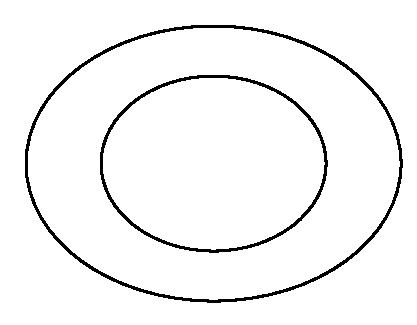
\includegraphics[scale=0.6]{Figures/fig1}
\end{center}
\caption{Lorsque $d=4$, un ovale peut être dans un autre}\label{fig1}
\end{figure}

Mais le cas suivant est impossible :
\begin{figure}[H]
\begin{center}
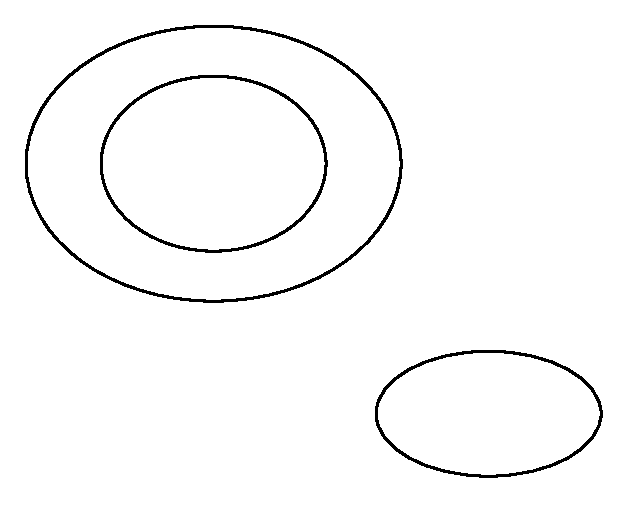
\includegraphics[scale=0.6]{Figures/fig2}
\end{center}
\caption{Ceci est impossible}
\end{figure}
En effet, si nous traçons une droite qui coupe chacun des ovales en deux points, nous obtenons $6$ points d'intersections alors que le degré de l'équation sous-jacente est de $4$.
\begin{figure}[H]
\begin{center}
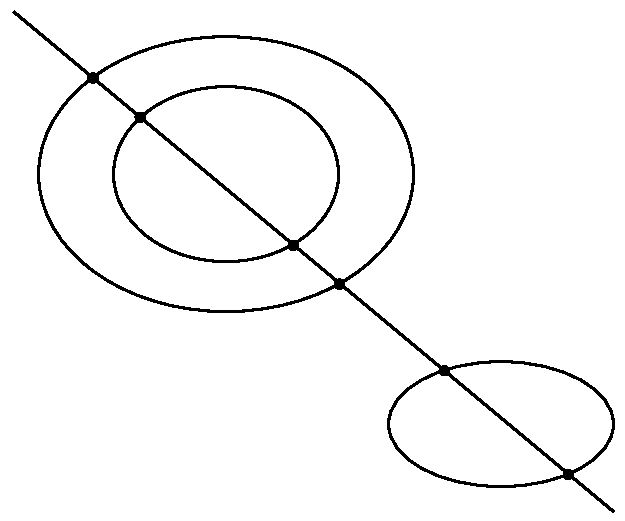
\includegraphics[scale=0.55]{Figures/fig3}
\end{center}
\caption{Les six points d'intersections contredisent $d=4$}
\end{figure}

Nous procédons de même avec le cas où nous aurions $5$ ovales. Par leurs $5$ centres passe une conique et l'intersection est de $10$ points alors qu'il devrait y en avoir au plus $4\times 2 = 8$.


\mainmatter

\chapter{Géométrie des courbes algébriques}

\section{Lemme de \textsc{Morse}}

D'après \textsc{Milnor}, \emph{Morse Theory}.
\lemme{ 
Soit $p$ un point critique non dégénéré de $f$. Alors il existe un système de coordonnées locales $(y^{1},\ldots,y^{n})$ dans un voisinage $U$ de $p$ tel que $y^{i}(p)=0$ pour tout $i$ et aussi : \[ f= f(p) - (y^{1})^{2} -\ldots - (y^{\lambda})^{2} + (y^{\lambda+1})^{2} + \ldots + (y^{n})^{2}  \]avec $\lambda$ l'index de $f$ en $p$.
}{\textsc{Morse}}

Nous commençons par se donner un lemme préliminaire :

\lemme{
Si $f$ est lisse dans un voisinage $V$ de $0\in \R^{n}$ avec $f(0)=0$ alors \[ f(x^1,\ldots,x^n) = \sum_{i=1}^{n}x^ig_i(x^1,\ldots,x^n)\]avec des fonctions $g_i$ lisse sur $V$ et telles que\[g_i(0) = \frac{\partial f}{\partial x^{i}}(0). \]
}{}
\preuve{
Nous avons l'égalité \[f(x) = \int_{0}^{1} \frac{\dd f(tx) }{\dt}\dt = \int_{0}^{1}\sum_{i=1}^{n}\frac{\partial f}{\partial x^{i}}(tx)\cdot x^{i}\dt \]et nous définissons alors \[g_i(x) = \int_{0}^{1}\frac{\partial f}{\partial x^{i}} (tx)\dt.\]
}{}


\preuve{ 
Nous commençons par montrer que si $f$ a une telle expression alors $\lambda$ est l'index de $f$ en $p$. Supposons ainsi pour un systèmes de coordonnées $(z^{1},\ldots,z^{n})$ que \[ f(q) = f(p) - (z^{1}(q))^{2} - \ldots - (z^{\lambda}(q))^{2} + (z^{\lambda+1}(q))^{2} + \ldots + (z^{n}(\lambda))^{2}. \]Alors \[ \frac{\partial^{2} f}{\partial z^{i}\partial z^{j}}(p) = \systeme{-2 &\text{ si }i=j\leq \lambda \\ 2& \text{ si }i=j>\lambda \\0 &\text{ sinon}.}  \]

Cela montre que la matrice de $\Delta f$ selon la base $\displaystyle\der{}{z^{1}}{p},\ldots,\der{}{z^{n}}{p}$ est diagonale avec $\lambda$ fois $-2$, $(n-\lambda)$ fois $2$ sur la diagonale et dans cet ordre.

Ainsi, il existe un sous-espace de $\rT M_p$ de dimension $\lambda$ où $\Delta f$ est définie négative et un sous-espace de dimension $n-\lambda$ où $\Delta f$ est définie positive. Cela montre que $\lambda$ est l'index de $f$ en $p$.

Il nous reste à montrer qu'un tel système de coordonnées existe. Pour cela, nous commençons par supposer que $p=0$ et $f(0)=0$, par le lemme précédent nous obtenons des $g_i$ telles que \[ f(x) = x^{i}g_i(x) .\]Comme $0$ est un point critique, $g_i(0)=0$ pour tout $i$ et donc il existe des $h_{i,j}$ telles que \[f(x) = x^{i}x^{j}h_{i,j}(x). \]Nous pouvons supposer (quitte à moyenner) que $h_{i,j}=h_{j,i}$.

Pour obtenir le système de coordonnées, nous allons imiter la preuve de diagonalisation des formes quadratiques. Procédons par récurrence, supposons qu'il existe $u^{1},\ldots,u^{n}$ définies dans un voisinage $U_1$ de $0$ telles que \[f = \pm(u^{1})^{2} \pm \ldots \pm (u^{r-1})^{2} + \sum_{i,j\geq r}u^{i}u^{j}H_{i,j}(u^{1},\ldots,u^{n})\]sur $U_1$ et où la matrice  décrite par $H_{i,j}(u^{1},\ldots,u^{n})$ (de taille $(n-r+1)\times (n-r+1)$) est symétrique. Après un changement linéaire sur la dernière coordonnée, on peut faire en sorte que $H_{r,r}(0)\neq 0$. Désignons par $g(u^{1},\ldots,u^{n})$ la racine carrée de $|H_{r,r}(u^{1},\ldots,u^{n})|$. Comme $g$ est non nulle en $0$ et est lisse, il existe un voisinage $U_2\dans U_1$ de $0$ où $g$ est non nulle. On pose $v^{i}=u^{i}$ pour $i\neq r$ et \[ v^{r}(u^{1},\ldots,u^{n}) = g(u^{1},\ldots,u^{n})\left(u^r + \sum_{i>r}u^i \frac{H_{i,r}(u^{1},\ldots,u^{n})}{H_{r,r}(u^{1},\ldots,u^{n})}\right).   \]
Par le théorème d'inversion locale, $(v^{1},\ldots,v^{n})$ sera un système de coordonnées dans un voisinage $U_3\dans U_2$ de $0$. Cela complète la récurrence puisque sur $U_3$ : \[ f = \pm(v^{1})^{2} \pm \ldots \pm (v^{r})^{2} + \sum_{i,j>r}v^{i}v^{j}H_{i,j}(v^{1},\ldots,v^{n}).  \]

}{Lemme de \textsc{Morse}}


\section{Théorème des petites perturbations}

\definition{ 
Nous dirons que $\xi=(\xi_1,\xi_2,\xi_3)$ est un \emph{croisement} si $\Delta P(\xi)$ a une valeur propre positive et une négative.
}{}

De manière équivalente, $\xi$ est un croisement si $\xi$ est un point critique non dégénéré et d'index $1$ pour les applications : \[\fonc{\varphi_i}{\ens{x_i\neq 0}}{\R}{x}{\frac{P(x)}{x_i}\deg P} \]pour $i$ tel que $\xi_i\neq 0$.

Le lemme de \textsc{Morse} implique qu'au voisinage de $\xi$, $\R P$ est la réunion de deux droites réelles.

Réciproquement, si $\R A_1, \ldots, \R A_k$ sont non singulières, mutuellement transverse et si $3$ d'entre-elles ne se croisent jamais, alors les points critiques de $\R A_1 \cup \cdots \cup \R A_k$ sont des croisements.

Le théorème des petites perturbations s'énonce de la manière suivante :

\theoreme{ 
Soient $P$ et $Q$ deux polynômes de degré $n$ et tels que $\R Q$ ne passe pas par les points critiques de $\R P$. Soit $U$ un voisinage régulier de $\R A$ dans $\P^{2}(\R)$ tel que $U$ se décompose selon : \[U = U_0 \sqcup U_1 \]où $U_0$ est voisinage des points critiques et $U_1$ est un voisinage tubulaire de la sous-variété $\R P-U_0$.

Alors il existe $X$ de degré $n$ tel que :
\begin{enumerate}
\item la courbe $\R X$ est partie de $U$ ;
\item pour chaque composante connexe $V$ de $U_0$, il existe un homéomorphisme $h:V\to D^{1}\times D^{1}$ (avec $D^{1}$ le disque unité de dimension $1$) tel que : \[ h(\R P \cap V) = D^{1}\times \{0\}, \; h(\R Q\cap V) = \{0\} \times D^{1},\]\[ h(\R X \cap V) = \ens{xy = \frac{1}{2}}\dans D^{1}\times D^{1} \, ; \]
\item $\R X -U_0$ est une section du fibré tubulaire $V_1 \to \R P-U_0$ ; 
\item $\R X$ est partie de $\ens{P(x_0,x_1,x_2)Q(x_0,x_1,x_2) \leq 0}$ ;
\item $\R X \cap \R P = \R X \cap \R Q = \R P \cap \R Q$ ;
\item si $p\in \R P\cap \R Q$ est non singulier de $Q$ et si $\R Q$ est transverse à $\R P$ en $p$ alors $\R X$ est transverse à $\R Q$ en $p$.
\end{enumerate}
Il existe aussi $\eps >0$ tel que pour tout $t\in ]0,\eps]$, $X=P+tQ$ convienne.
}{}



\end{document}
